\subsection{Módulo genérico de los cambios en tijeras}
	\label{sec:ACG_scr}
		
	El módulo \textit{ScissorCrossings} es el encargado de implementar el funcionamiento de los cambios de vías en tijeras en la red ferroviaria. Su implementación es similar a la del módulo \textit{SingleSwitches}, con el ACG utilizando la información otorgada por el RNA para implementar las entradas y salidas necesarias para habilitar el movimiento del cambio de vías solo en situaciones seguras y confirmando su correspondencia mediante la comparación del comando y la indicación. El diagrama de bloques de las máquinas de estado finitas con camino de datos diseñado para lograr este objetivo se muestra en la Figura \ref{fig:SCR_module}.
	
	\begin{figure}[H]
		\centering
		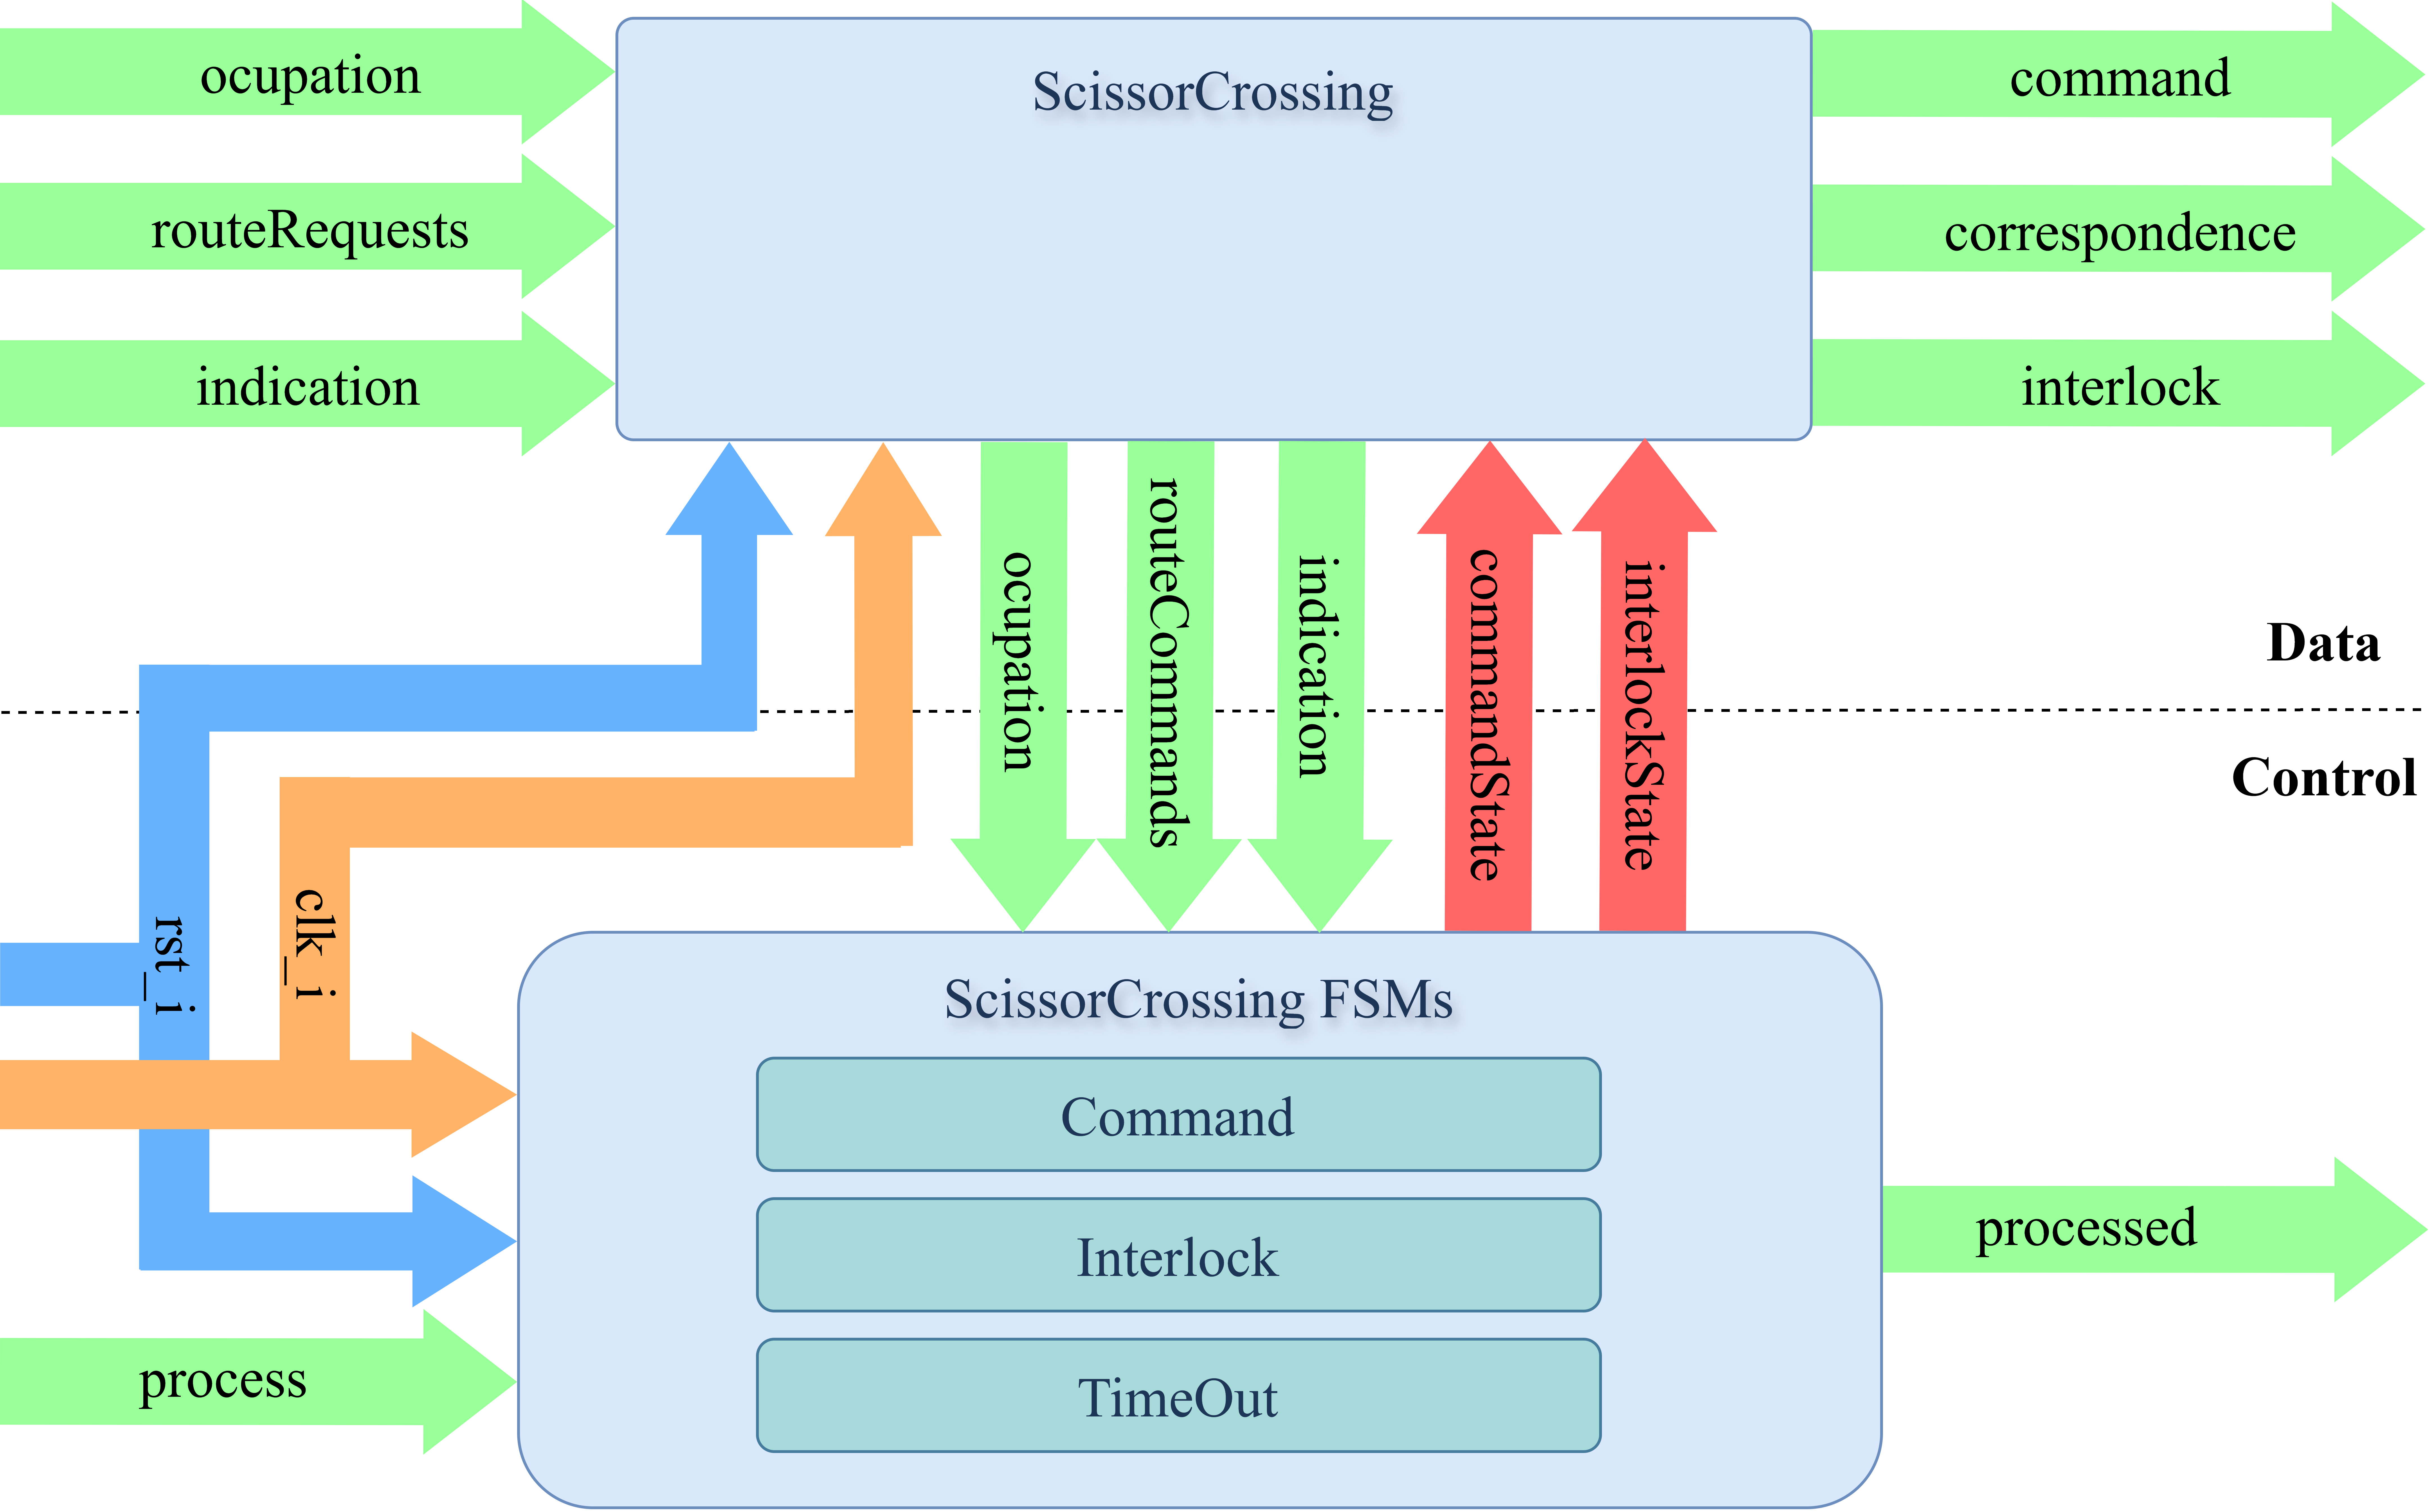
\includegraphics[width=1\textwidth]{Figuras/SCR_module}
		\centering\caption{FSMD del módulo genérico de \textit{ScissorCrossings}.}
		\label{fig:SCR_module}
	\end{figure}
	
	Tal se explicó en la Sección \textit{SingleSwitches}, los cambios de vías en tijeras tienen dos posiciones estables: normal y reversa. A diferencia de los cambios de vías simples, donde la posición normal es la posición de mayor prioridad, ya que permite la circulación por vía principal; los posiciones en los cambios de vías en tijeras tienen igual prioridad, ya que ambas posiciones permiten la circulación por vías de igual categoría, pudiendo ser ambas principales. Por lo tanto, aun cuando por defecto se mantiene la funcionalidad de que un cambio de vías retorne a su posición original luego de llegar al timeout sin poder concretar el movimiento, esta función puede desactivarse y dejar el cambio en una posición intermedia luego de un timeout. El comportamiento de los cambios de vías dobles es mucho más complejo, tal como se define en la red de Petri de la Figura \ref{fig:DSW_Petri}.
	
	\begin{figure}[H]
		\centering
		\includegraphics[width=1\textwidth]{Figuras/SSW_Petri}
		\centering\caption{Red de Petri del modelo dinámico de \textit{ScissorCrossings}.}
		\label{fig:SCR_Petri}
	\end{figure}
	
	En definitiva, los cambios de vías presentan diferencias en sus modelos dinámicos de comportamiento y en el tamaño de los puertos de comando, indicación y correspondecia, pero a grandes rasgos presentan muchas similitudes que son aprovechadas por el ACG. Entre las ventajas encontradas tenemos el uso de una plantilla común a la hora de definir los módulos y sus máquinas de estados, agilizando el proceso de desarrollo del ACG. Además, ésto facilita la comprobación y validación de los módulos al compartir raíces comunes.
